\documentclass[main.tex]{subfiles}

\begin{document}

\section{References}


\paragraph{Analytical solutions for Newtonian and inelastic non-Newtonian flows with wall slip }\cite{ferrasAnalyticalSolutionsNewtonian2012}
In this articles they propose analytical solutions for the Couette and Poiseuille flow with slip Boundary conditions of steady, incomprehensible, laminar flow.
The momentum equation is,
\begin{gather*}
	\pdv{y}\qty(\eta\qty(\dot\gamma)\pdv{u}{y}) = \pdv{p}{x}.
\end{gather*}
The slip laws that they analyze are, 
\begin{align*}
	\mathrm{Linear~Navier~slip~law} &: u_ws = \overline k\left.\frac{du}{dy}\right|_{wall}, \\
	\mathrm{Non-linear~Navier~slip~law} &:  u_{ws} = \mathrm{sign}\left(\frac{du}{dy}\right)\frac{\overline k}{\eta(\dot\gamma)}\left|\tau_{xy}\right|^{m-1}\tau_{xy} \\
	\mathrm{Hatzikiriakos} &: u_{ws} = \left\{ 
	\begin{array}{ll}
		k_1\sinh\left(k_2\left(\mathrm{sign}\left(\frac{du}{dy}\right)\tau_{xy}\right)-\tau_{c}\right) & \tau_{xy}\geq\tau_{c} \\
		0 & \tau_{xy}<\tau_{c}
	\end{array}
	\right. \\
	\mathrm{Asymptotic} &: u_{ws} = k_1\ln\left[ 1+k_2\left(\mathrm{sign}\left(\frac{du}{dy}\right)\tau_{xy}\right) \right].
\end{align*}
Finally, also they take into account Non-Newtonian fluids with the following constitutive equations:
\begin{align*}
	\mathrm{Power~Law} &: \eta\qty(\dot\gamma) = a\qty(\dv{u}{y})^{n-1}, \\
	\mathrm{Sisko} &: \eta(\dot{\gamma}) = \mu_{\infty} + a\left|\dot{\gamma}\right|^{n-1}, \\
	\mathrm{Herschel-Bulkley~(Bingham)} &: \mu\qty(\dot\gamma) = \left\{
	\begin{array}{ll}
		\frac{\tau_o}{\abs{\dot\gamma}}+k\abs{\dot\gamma}^{n-1} & \abs{\dot\gamma}\geq\dot\gamma_o\\
		\mu_o & \abs{\dot\gamma}\leq\dot\gamma_o
	\end{array}
	\right.
\end{align*}

\paragraph{Inhomogeneous Coutte-Poiseuille shear flow}\cite{gorulevaInhomogeneousCouettePoiseuille2022}
In this article an exact solution for the Navier-Stokes equations for steady-state flow of a viscous in-compressible fluid is presented, describing a fluid flow in a thin layer, which can be treated as a large flow of vertical vortex fluid without prerotation.

\paragraph{A review of methods on buildability quantification of extrusion-based 3D concrete printing from analytical modeling to numerical simulation.}\cite{changReviewMethodsBuildability2023}
In this article they give an overview of the following stages of 3D concrete printing: pumping extrusion and Build-up.
Then, they present a collection of experimental, analytical and numerical methods to quantify buildability.
The article concludes that 
The rheological models can investigate the material failure during the printing process from the perspective of chemical reaction and physical origin.
A reliable numerical model can be utilized to investigate the structural behavior and optimize the printing parameters and material design.
There are two typical printing model: laminar flow and non-laminar flow and the principal difference of the existence of compressive force from the nozzle.
All propoosed numerical methods have limited applications.
Finally, due to the relative simplicity of current 3D printing models, almost all the reviewed models only take the time-dependent stiffness and strength into account for buildability quantification. 
The time-dependent behaviours such as early-age creep and shrinkage may also significantly affect structural buildability and should be analyzed.



\paragraph{Newtonian Poiseuille flow in ducts of annular-sector cross-sections with Navier slip}\cite{kyritsi-yiallourouNewtonianPoiseuilleFlow2018}
In this article they propose a general analytical solution of a Newtonian Poiseuille flow in a duct with circular or annular cross section, using Navier slip in both walls and only in the outer wall.
They assume a flow unidirectional driven by a constant pressure-gradient in the absence of gravity,
\begin{gather*}
	-\pdv{p}{z}+\eta\qty(\pdv[2]{u}{r}+\frac{1}{r}\pdv{u}{r}+\frac{1}{r^2}\pdv[2]{u}{\theta}) = 0.
\end{gather*}
\begin{figure}[ht]
	\begin{subfigure}[c]{0.45\textwidth}
		\centering
		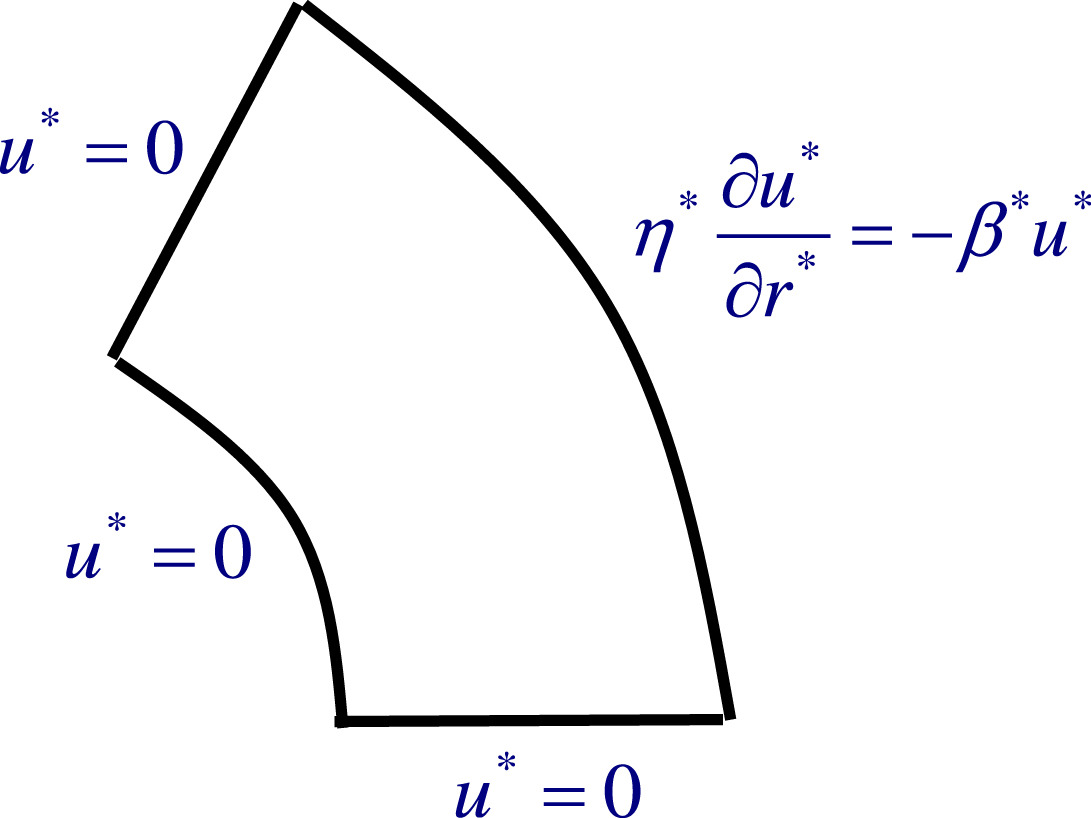
\includegraphics[width=\textwidth]{imgs/newtonPoiseuilleflowinductsofAnnularsectorCrosssectionwithNavierSlipimg1.jpg}
	\end{subfigure}
	\hfill
	\begin{subfigure}[c]{0.45\textwidth}
		\centering
		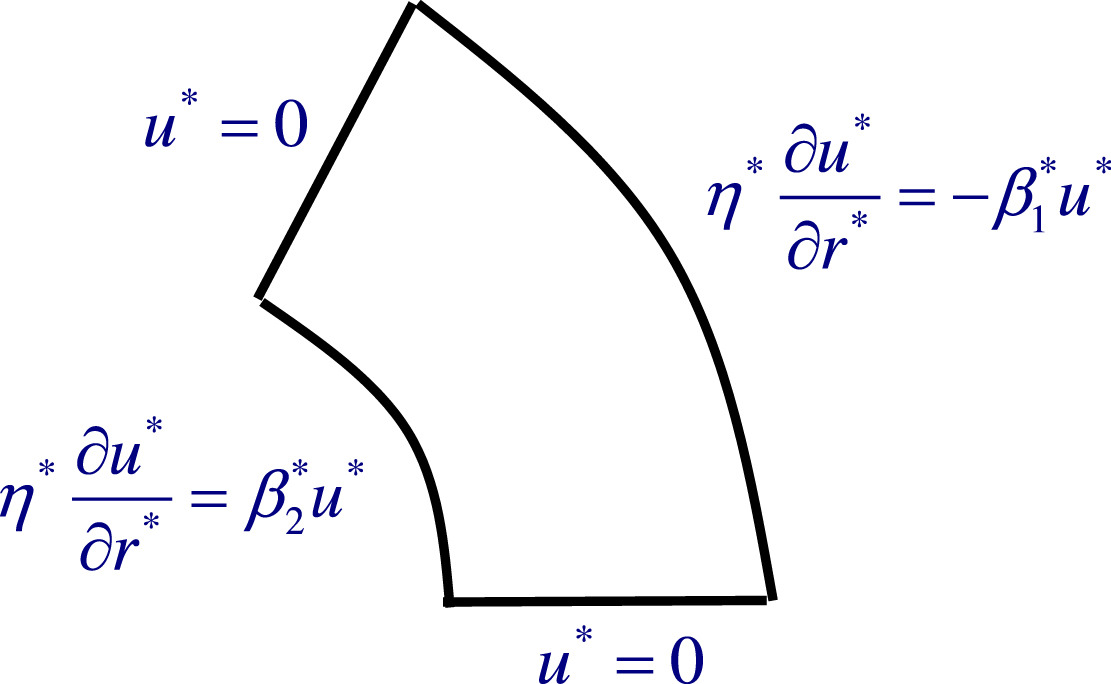
\includegraphics[width=\textwidth]{imgs/newtonPoiseuilleflowinductsofAnnularsectorCrosssectionwithNavierSlipimg2.jpg}
	\end{subfigure}
\end{figure}


\paragraph{Newtonian Poiseuille flows with slip and non-zero slip yield stress}\cite{kaoullasNewtonianPoiseuilleFlows2013}
In this article an analytical solution for the steady, incompressible Newtonian Poiseuille flow assuming thet slip occurs along the wall, following a Navier-type slip law with a non-zero slip yield stress in a rectangular, axisysmmetric and annular configurations.
The boundary slip condition is given by,
\begin{gather*}
	u_w = \left\{
		\begin{array}{ll}
			0, &\quad \tau_w\leq\tau_c \\
			\frac{1}{\beta}\qty(\tau_w-\tau_c), &\quad\tau_w>\tau_c.
		\end{array} 
	\right.
\end{gather*}
They  analyze a steady creeping, pressure-drive flow of a n incompressible Newtonian fluid with zero gravity.
For the rectangular geometry,
\begin{gather*}
	\pdv[2]{u_x}{y} + \pdv[2]{u_x}{z} = -\frac{1}{\eta}\pdv{p}{z},
\end{gather*}
and for the axissymmetric and annular configurations,
\begin{gather*}
	-\pdv{p}{z}+\eta\qty(\pdv[2]{u_z}{r}+\frac{1}{r}\pdv{u_z}{r})=0.
\end{gather*}


\paragraph{Stability of the annular Poiseuille flow of a Newtonian liquid with slip along the walls}\cite{chatziminaStabilityAnnularPoiseuille2009}
In this article they analyze the solutions of the annular Poiseuille flow of a Newtonian fluid assuming that slip occurs along the walls.
The slips that they consider are, lnear, piecewise linear and three branch.


\paragraph{Viscoplastic Poiseuille flow in a rectangular duct with wall slip.}\cite{damianouCessationViscoplasticPoiseuille2014}
They solve numerically and analytically the Poiseuille flow of a Herschel–Bulkley fluid in a duct of rectangular cross section under the assumption that slip occurs along the wall following a slip law involving a non-zero slip yield stress.
Steady-state flow,
\begin{gather*}
	\pdv[2]{u_x}{y} + \pdv[2]{u_x}{z} = -\frac{1}{\eta}\pdv{p}{z},
\end{gather*}
and use the Navier law as boundary condition,
\begin{gather*}
	\tau_w = \beta u_w.
\end{gather*}
They show that the regularization of the equations leads to accurate solutions for unyielded regions, provided that the regularization parameter is of the order of $10^6$ and higher.


\bibliography{MaestriaNanoII}


\end{document}